\documentclass[12pt,a4paper]{article}
\usepackage{graphicx} % Required for inserting images
\usepackage{tikz}
\usepackage[left=2.00cm, right=1.00cm]{geometry}
\usepackage{xcolor} % before tikz or tkz-euclide if necessary
\usepackage{amsmath}
\usepackage{siunitx}
\usepackage{chemfig}
\usetikzlibrary{calc}
\begin{document}
\begin{center}
    \large\textbf{Løsningsforslag til prøve i termodynamikk:}
\end{center}
1.  Hvordan er temperaturskalaen Kelvin definert?\\\\
Kelvinskalaen ble oppfunnet av William Thomson.  For dette arbeidet ble han Lord Kelvon (Kelvin er navnet på elven som renner ved universitet i Glasogaow der Thomson arbeidet som professor).   Noe forenklet forkalrt kom han frem til at ved en bestemt temperatur så har ikke molekylene bevegelse.  Han bestemte derfor at dette skulle være det absolute nullpunktet i temperaturskalaen. Ved å se på forsøk og matematikk kom han (antakeiig  is samarbeid med andre) frem til at dette tilsvarte $-273,k15^\circ C$. \\\\
2.  Hva menes med det absolutte nullpunkt?\\\\
Det absolutte nullpunktet er den laveste mulige temperaturen. Og den er $-273,15^\circ C$.\\\\
3. Hva sier den ideelle gasslov og hva er enhetene til de ulike verdiene?\\\\
Den ideelle gasslov:\\\\
$P\cdot V=n\cdot R\cdot T$\\\\
Der:\\\\
P=gassens trykk (Pa, $N/m^2$)\\
n=antall molekyl, eller stoffmengde (mol)\\
R=gasskonstanten (8,314J/molK)\\
V=gassens volum ($m^3)$\\
T=temperaturen i K (kelvin)\\\\
4.  Regn om til Kelvin:  $35 ^\circ C, 63^\circ C, -26^\circ C, 253^\circ C $\\\\
Formel: $T_k=T_C+273,15$\\
Vi får: 308,15K, 336,15K, 247,15K, 526,15K\\\\
5. Regn om til celisus: 273,15K, 233K, 57K, 800K\\\\
Formel: $T_C=T_K-273,15$\\
Vi får: $0^\circ C, -40,15^\circ C, -216,16^\circ C, 526,85^\circ C$\newpage

6. En gass innestengt i beholder har et trykk på $P_1=5,3bar$.  hvor stort blir trykket når vi halverer volumet og temperaturen er konstant? $V_1=6L$\\\\
Her bruker vi loven for konstant temperatur:\\
$$P_1\cdot V_1=P_2\cdot V_2$$\\
Her er $P_1=5,3bar$ og $V_1=6L$.  Vi halverer volumet, slik at $V_2=3L$. Vi skl finn slutt trykket, $P_2$.  Vi snur på formelen og får (bruk krysset):\\
$$P_2=\frac{P_1\cdot V_1}{V_2}=\frac{5,3bar\cdot 6L}{3L}=10,6bar$$
7.  Vi har gitt følgende stempel med en gass som er innestengt.  Vi har et stempel som vi kan skyve inn og ut:\vspace{0.5cm}\\
\begin{center}
    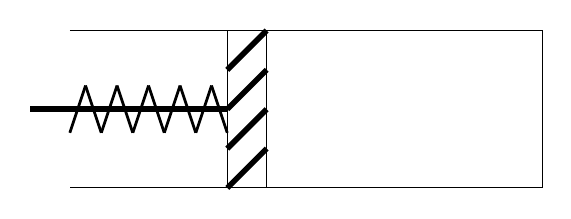
\begin{tikzpicture}
        %stempel med variabel
        \pgfmathsetmacro{\myLength}{4}
        \draw (2,2)--(8,2)--(8,0)--(2,0);
        \draw (\myLength,0)--(\myLength+0.5,0)--(\myLength+0.5,2)--(\myLength,2)--(\myLength,0);
        \draw [line width=2pt] (\myLength,0)--(\myLength+0.5,0.5);
        \draw [line width=2pt] (\myLength,0.5)--(\myLength+0.5,1);
        \draw [line width=2pt] (\myLength,1)--(\myLength+0.5,1.5);
        \draw [line width=2pt] (\myLength,1.5)--(\myLength+0.5,2);
        \draw [line width=2pt] (\myLength,1)--(\myLength-2.5,1);
        \draw [line width=1pt] (2,0.7)--(2.2,1.3);
        \draw [line width=1pt] (2.2,1.3)--(2.4,0.7);
        \draw [line width=1pt] (2.4,0.7)--(2.6,1.3);
        \draw [line width=1pt] (2.6,1.3)--(2.8,0.7);
        \draw [line width=1pt] (2.8,0.7)--(3.0,1.3);
        \draw [line width=1pt] (3.0,1.3)--(3.2,0.7);
        \draw [line width=1pt] (3.2,0.7)--(3.4,1.3);
        \draw [line width=1pt] (3.4,1.3)--(3.6,0.7);
        \draw [line width=1pt] (\myLength-0.4,0.7)--(\myLength-0.2,1.3);
        \draw [line width=1pt] (\myLength-0.2,1.3)--(\myLength,0.7);
    \end{tikzpicture}
\end{center}\vspace{1cm}
I starten er volumet $V_1=8L$ og trykket er lik $P_1=2,1bar$ .  Vi endrer volumet mens temperaturen er konstant slik at volumet blir $V_2=2L$.  Hva blir det nye trykket $P_2?$ \\\\
Denne oppgaven er egenltig helt lik oppgave 6. Siden temperaturen er konstant bruker vi gassloven for konstant temperatur:\\
$$P_V\cdot V_1=P_2\cdot V_2$$
Løst m.h.p. $P_2$ (bruk krysset):

$$P_2=\frac{P_2\cdot V_1}{V_2}=\frac{2,1bar\cdot 8L}{2L}=8,4bar$$\newpage
8.  Temperaturen til gassen er nå $T_2=52^\circ C$.  Vi øker temperaturen til $T_3=400K$.  Hva blir det nye trykket $P_3$ om vi antar at volumet er konstant?\\
I dette tilfellet er det volumet som er konstant.  Da er det følgene ligning som gjelder:\\
$$\frac{P_2}{T_2}=\frac{P_3}{T_3}$$
Vi bruker "krysset" for å finne $P_3$:
$$P_3=\frac{P_2\cdot T_3}{T_2}=\frac{8,4bar\cdot 400K}{(52+273,15)K}=\frac{8,4bar\cdot 400K}{325,15K}=10,3bar$$\\
9. Vi kan se på en firkantet kloss som ligger på et bord:\\\\\\\
\begin{center}
    \begin{tikzpicture}[scale=0.8]
        \draw (4,0)--(4,4);
        \draw (2,4)--(10,4);
        \draw (8,0)--(8,4);
        \draw (5,4) rectangle (7,6);
    \end{tikzpicture}    
\end{center}
Denne klossen har en masse 1,83kg og et areal som berører bordplaten.  Den yter dermedet trykk P mot bordet.  Sidene er lengde lik 30cm (0,3m), høyde lik 15cm (0,15m) og bredde lik 20cm (0,2m):\\
\begin{tikzpicture}[scale=1.5,transform canvas={shift={(6cm,-3cm)}}]


% Dimensjoner
\def\L{4}   % lengde
\def\B{2}   % bredde (dybde)
\def\H{1}   % høyde

% Vektor for dybde (perspektiv)
\coordinate (D) at (-0.5,0.3);

% Bunnflate
\draw (0,0) -- (\L,0) -- ++(D) -- ++(-\L,0) -- cycle;

% Vertikale kanter (høyde)
\draw (0,0) -- ++(0,\H);
\draw (\L,0) -- ++(0,\H);
\draw ($(0,0)+ (D)$) -- ++(0,\H);
\draw ($( \L,0) + (D)$) -- ++(0,\H);

% Toppflate
\draw (0,\H) -- (\L,\H) -- ++(D) -- ++(-\L,0) -- cycle;

% Linjer bakover (dybde)
\draw (\L,0) -- ++(D);
\draw (\L,\H) -- ++(D);
\node at (2,1.5) {lengde=30cm (0,3m)};
\node at (5.5,0.5) {høyde=15cm (0,15m)};
\node at (-1.8,0.2) {bredde=20cm (0,2m)};
\end{tikzpicture}\\
\vspace{4cm}
\\Denne klossen kan plasseres på tre forskjellig måter på bordet.  Beregn de tre ulike trykkene som klossen yter mot bordflaten.\newpage
\noindent\textbf{Svar:}\\
Denne klossen kan plasseres på tre forskjellig måter på bordet.  Og de vil gi ulikt trykke mot bordet. For arealet vil variere.  Vi beregner arealene, og gjør om til meter:\\
areal 1: lengde 30cm, bredde 20cm:  $A_1=0,3m\cdot 0,2m=0,06m^2$\\
areal 2: lengde 30cm, bredde 15cm:  $A_1=0,3m\cdot 0,15m=0,045m^2$\\
areal 3: lengde 20cm, bredde 15cm:  $A_1=0,2m\cdot 0,15m=0,03m^2$\\\\
Vi er nå klare for å beregne de 3 trtyhkkene  Vi tar da utgangspunkti definisjonen for trykk:
$$P=\frac{F}{A}$$
der:\\
P=trykk ($N/m^2, Pa (Pascal)$\\
F=kraft (N, Newton)\\
A=Areal ($m^2$)\\

\noindent Kraften vi skal finne her  er lik tyngdekraften $G=m\cdot g$\\  
her er:\\
G=Tyngdekraften (N)\\
m=klossens masse (kg)\\
g=tyngdens akselerasjon ($N/m^2$)\\\\
\noindent Vi beregner trykkene nå når massen til klossen er 1,83kg:\\
$$P_1=\frac{G}{A_1}=\frac{1,83kg\cdot 9,8m/s^2}{0,06m^2}=298,9N/m^2$$\\
$$P_2=\frac{G}{A_2}=\frac{1,83kg\cdot 9,8m/s^2}{0,045m^2}=398,5N/m^2$$\\
$$P_3=\frac{G}{A_3}=\frac{1,83kg\cdot 9,8m/s^2}{0,03m^2}=597,8N/m^2$$

\end{document}